\section{Sampling Catalan Objects}%
\label{sec:catalan_objects}
\todo{Computing $p_d$ values. Mention that this is imperfect sampling (close impl.)}
\todo{Thresholding.}
\todo{Mention that this is imperfect sampling (close impl.)}
\todo{Fix $\sqrt{B\log n}$ everywhere.}

Earlier, we were interested in querying the following random object.
In a random permutation of $n$ white marbles and $n$ black marbles, how many white marbles are present in the first $k$ positions.
As we have seen before, \todo{we have?} \cite{huge} gives us a method of sampling from this (hypergeometric) distribution.
In constructing a generator for the Stochastic Block model, we generalized this by adding more colors (multivariate hypergeometric distribution).
We also took this to the extreme where all marbles are distinguishable (i.e. a random permutation),
and saw that this could also be implemented efficiently.
Now we focus on a more challenging variant of this question with more complicated conditional dependences among the placement of the marbles.
\todo{Connect with previous part on SBM}

\begin{figure}[htbp]
    \centering
    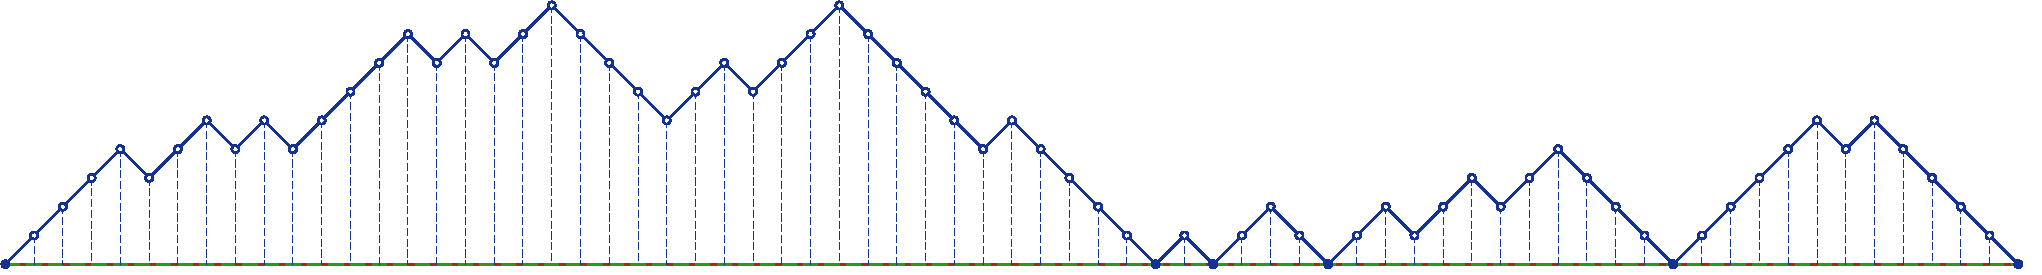
\includegraphics[width=\textwidth]{images/basic_dyck_path.pdf}
    \caption{Simple Dyck path with $n = 35$.}
    \label{fig:basic_dyck}
\end{figure}
We consider a sequence of $n$ white and $n$ black marbles such that every prefix of the sequence has at least as many white marbles as black ones.
The number of such is sequences is the $n^{th}$ Catalan number $C_n$.
Many important combinatorial objects occur in Catalan families.
Dyck paths are one such interpretation of the Catalan numbers that fits in nicely with our setup of white and black marbles.
A Dyck path is constructed as a $2n$ step one-dimensional walk with exactly $n$ up and down steps.
In Figure~\ref{fig:basic_dyck}, each step in the walk moves one unit along the positive $x$-axis and one unit up or down the positive $y$-axis.
Given these restrictions, we would obtain a 1D random walk pinned to zero  on both sides.
A Dyck path also has a restriction that the $y$-coordinate of any point on the random walk is $\ge 0$ i.e. the walk never crosses the $x$-axis.
The number of possible Dyck paths (see Theorem~\ref{thm:number_of_dyck_paths}) is the $n^{th}$ Catalan number $C_n=\frac{1}{n+1}\cdot{2n\choose n}$.

We will attempt to support queries to a uniformly random instance of a Dyck path.
Specifically, we will want to answer the following queries:
\begin{itemize}
    \item \func{Height}$(i)$: Returns the position of the path after $i$ steps
    \item \func{First-Return}$(i)$: Returns an index $j>i$ such that $\func{Height}(j)=\func{Height}(i)$ and for any $k$ between $i$ and $j$,
    $\func{Height}(k)$ is strictly greater than $\func{Height}(i)$.
\end{itemize}



\subsection{Bijections to other Catalan objects}%
\label{sec:bijections_to_other_catalan_objects}
The $\func{Height}$ query seems natural for Dyck paths, but the $\func{First-Return}$ query is important in exploring other Catalan objects.
or instance, consider a random well bracketed expression i.e. an uniform distribution over the Dyck language.
One can construct a trivial bijection between Dyck paths and words in this language
by replacing up and down steps with opening and closing brackets respectively.
The $\func{Height}$ query corresponds to asking for the nesting depth at a certain position in the word,
and $\func{First-Return}(i)$ returns the position of the matching bracket for position $i$.

There is also a natural bijection between Dyck paths and rooted ordered trees by letting the path be a transcript of the DFS traversal of a tree.
Starting with the root, for each ``up-step'' we move to a new child of the current node, and for each ``down-step'', we backtrack towards the root.
Here, the $\func{Height}$ query returns the depth of a node and the $\func{First-Return}$ query can be used to find the \emph{next child} of a node.
\todo{Figure? Degree queries by repeated application.}

Moving forwards, we will focus on Dyck paths for the sake of simplicity.



\subsection{Catalan Trapezoids and Generalized Dyck Paths}
In order to sample Dyck paths locally, we will need to analyze more general Catalan objects
which correspond to numbers in the \textit{Catalan Trapezoid} (presented in \cite{trap}).
Let $C_k(n,m)$ be the $(n,m)^{th}$ entry of the Catalan trapezoid of order $k$, where $C_1(n,m)$ corresponds to the Catalan triangle.
We can interpret $C_k(n,m)$ as  the number of \emph{generalized} Dyck paths.
Specifically, we consider a sequence of $n$ up-steps and $m$ down-steps, such that the sum of any initial sub-string is not less than $1-k$.
This means that we start our Dyck path at a height of $k-1$, and we are never allowed to cross below zero (Figure~\ref{fig:complex_dyck}).
The total number of such paths is exactly $C_k(n,m)$.
For $k = 1$ and $n=m$, we obtain the definition of the simple Dyck path (Figure~\ref{fig:basic_dyck}).
Now, we state a result from \cite{trap} without proof
$$
C_k(n,m)=
\begin{cases}
{n+m}\choose m &0\le m<k\\
{{n+m}\choose{m}} - {{n+m}\choose{m-k}} &k\le m\le n+k-1\\
0 &m>n+k-1
\end{cases}
$$

\begin{figure}[htbp]
    \centering
    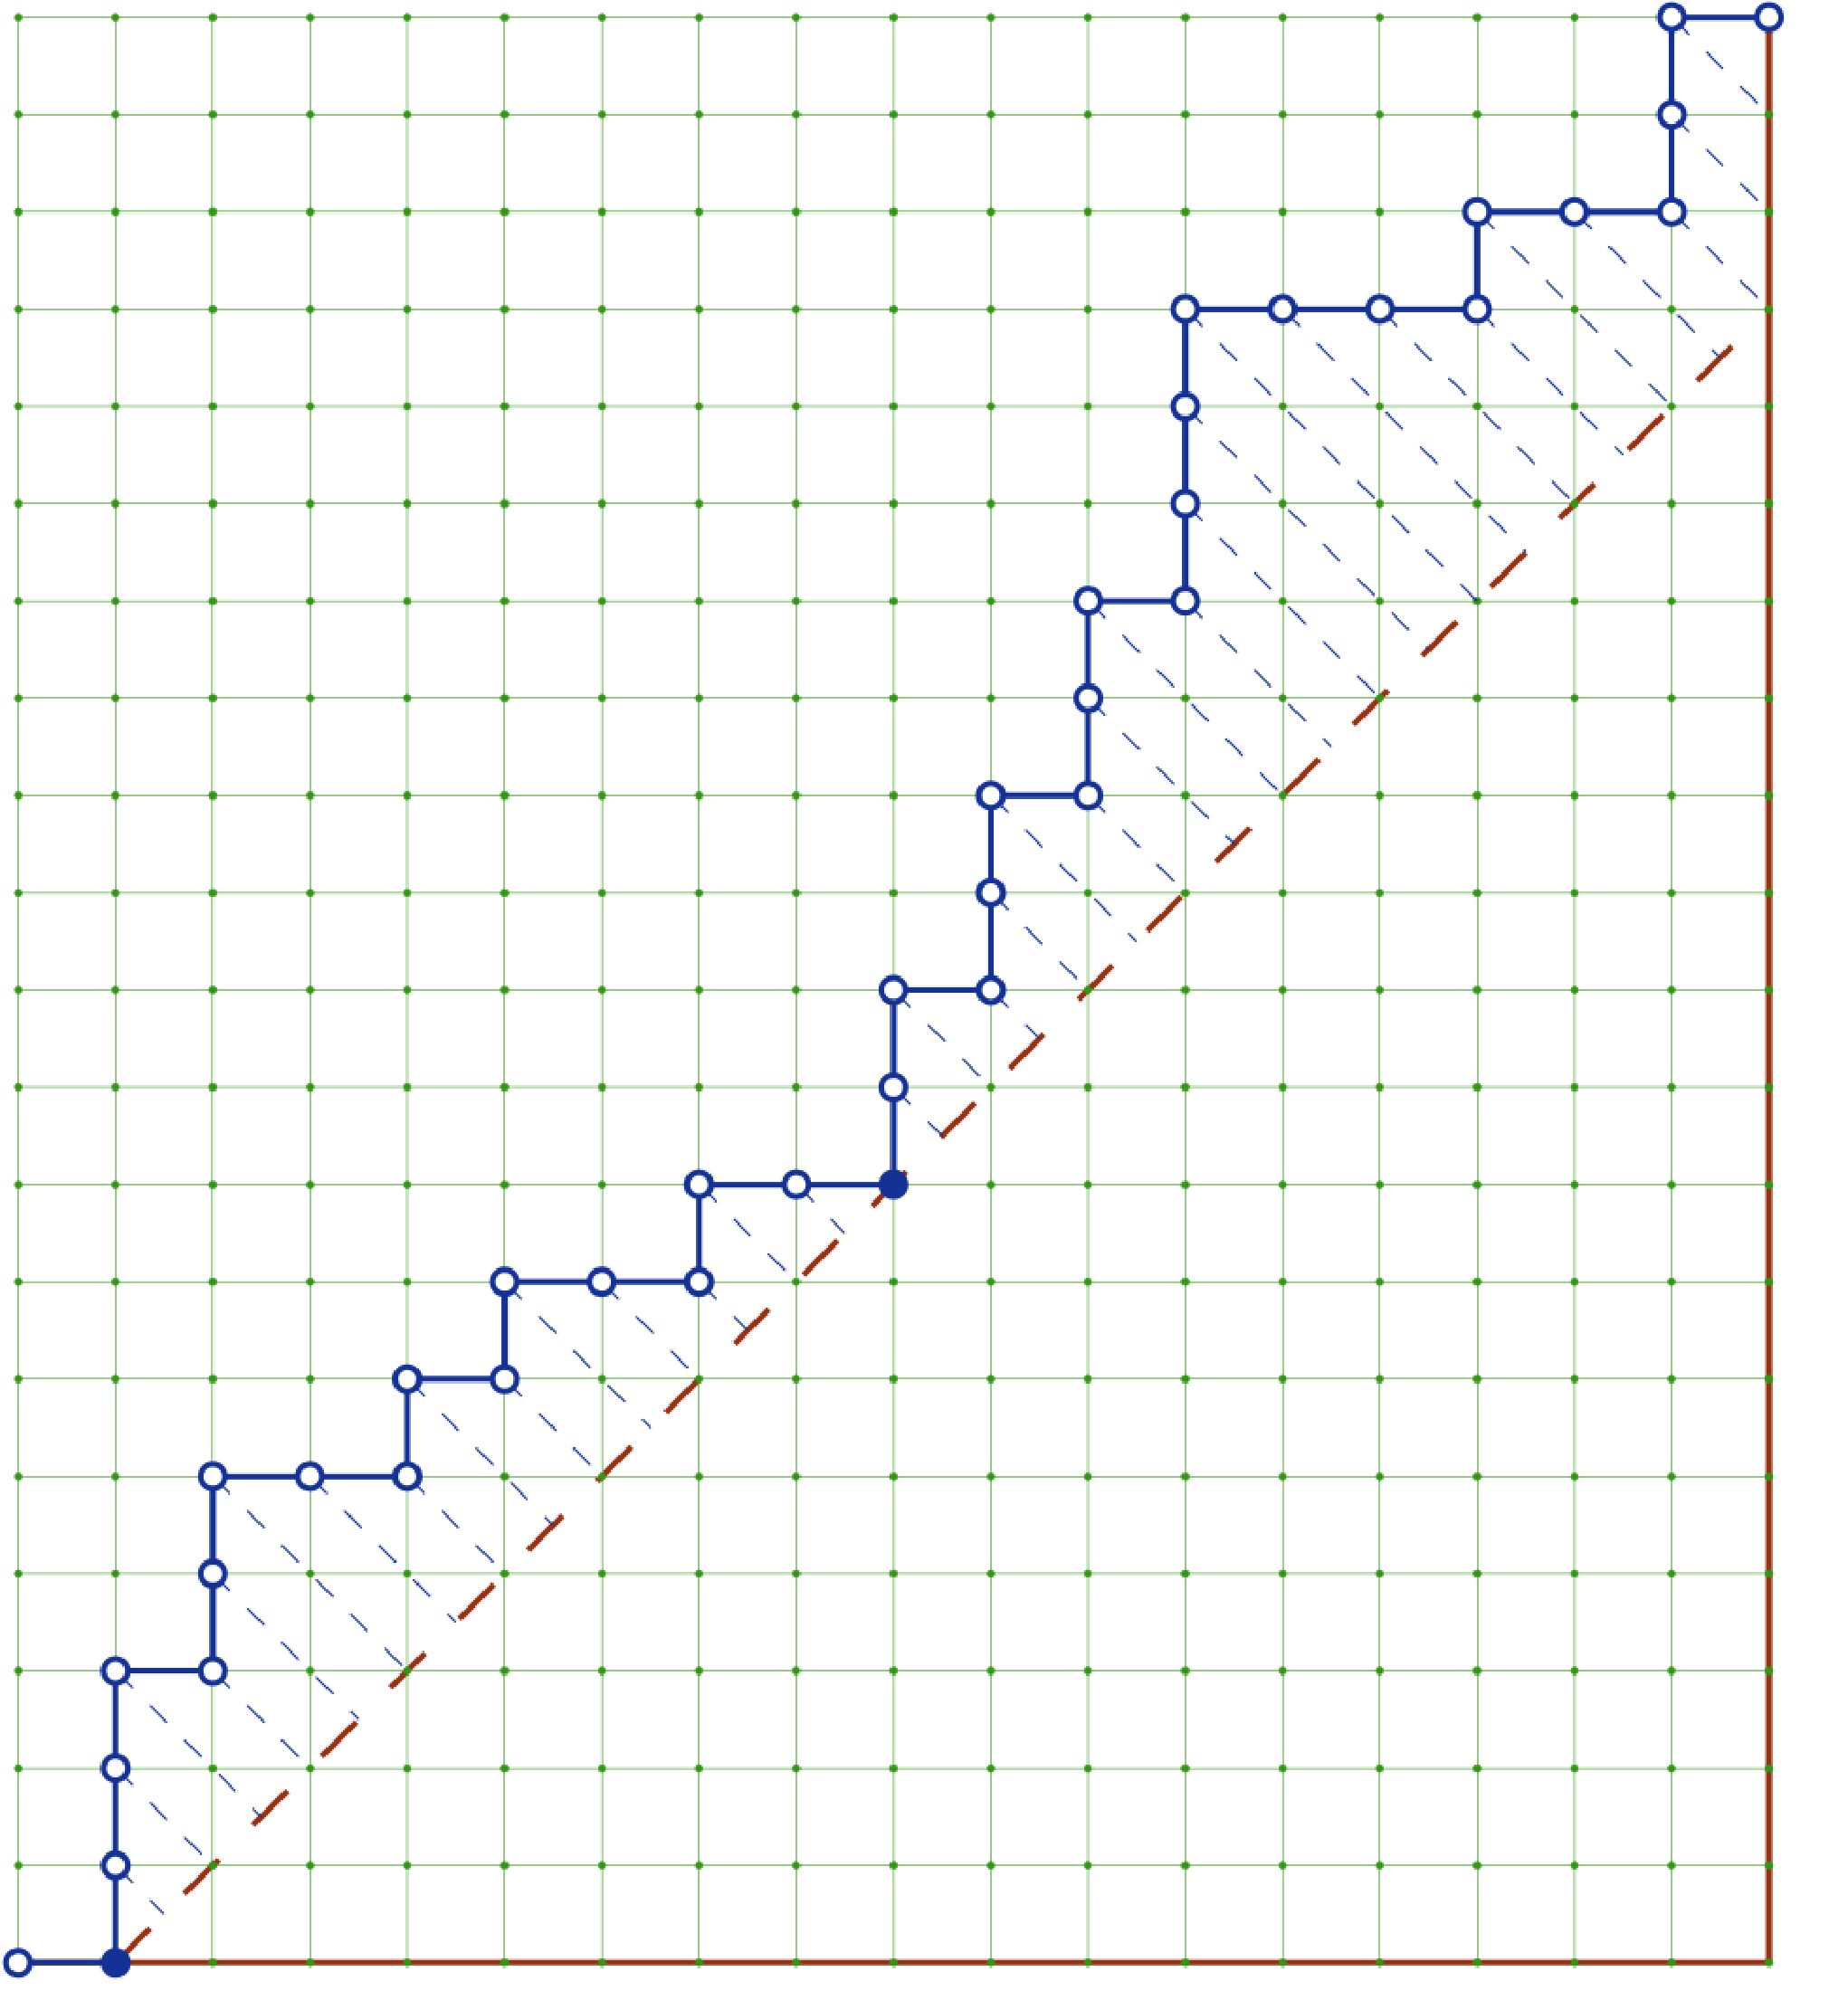
\includegraphics[width=\textwidth]{images/complex_dyck_path.pdf}
    \caption{Complex Dyck path with $n = 25$, $m = 22$ and $k = 3$.
             Notice that the boundary is shifted.} \label{fig:complex_dyck}
\end{figure}

\subsection{Sampling the Height}
Our general recursive step is as follows.
We consider a random sequence of length $2B$ comprising of $2U$ up steps ($+1$) and $2D$ down steps ($-1$)
where the sum of any prefix cannot be less than $k-1$.
Without loss of generality, let's assume that $2D\le B$. If this were not the case, we could simply flip the sequence and negate the elements.
This essentially means that the overall Dyck path is non-decreasing.

We want to sample the height of this path after $B$ steps.
This is the same as sampling the number of $(+1)$s that get assigned to the first half of the elements in the sequence.
We define $p_d$ as the probability that exactly $D-d$ $(-1)$s get assigned to the first half.
This means that exactly $U+d$ $(+1)$s get assigned to the first half.
Consequently, the second half will contain exactly $D+d$ $(-1)$s and $U-d$ $(+1)$s.
\todo{What is $d$ is negative?}


Let us first compute this probability.
$$
p_d = \frac{D_{left}\cdot D_{right}}{D_{tot}}
$$
Here, $D_{left}$ denotes the number of valid starting sequences (first half)
and $D_{right}$ denotes the number of valid ending sequences.
Here, \textit{valid} means that each half sequence gets the appropriate number of ups and downs
and the initial sums never drop below $1-k$.
For, $D_{right}$, we will start the Dyck path from the end of the $2B$ sequence.
In this case the invalidation threshold will be a different $k'$.
This $k'$ is the final height of the $2B$ sequence. So, $k'=k+2U-2D = k+4B-2D$.
We will use this fact extensively moving forward.

Also, $D_{tot}$ is the total number of possible sequences of length $2B$, given the initial conditions.
Note that in this case the threshold remains at $k$.

We will use the following rejection sampling lemma from \cite{huge}.
\todo{Frequently?}
\begin{lemma}
\label{lem:huge}
Let $\{p_i\}$ and $\{q_i\}$ be distributions satisfying the following conditions
\begin{enumerate}
    \item There is a poly-time algorithm to approximate $p_i$ and $q_i$ up to $\pm n^{-2}$
    \item Generating an index $i$ according to $q_i$ is closely implementable.
    \item There exists a $poly(log n)$-time recognizable set $B$ such that
    \begin{itemize}
        \item $1-\sum\limits_{i\in B} p_i$ is negligible
        \item There exists a constant $c$ such that for every $i$, it holds that $p_i\le \log^{\mathcal{O}(1)} n\cdot q_i$
    \end{itemize}
\end{enumerate}
Then, generating an index $i$ according to the distribution $\{p_i\}$ is closely-implementable.
\end{lemma}
An important point to note is that in order to apply this lemma, we must be able to compute the $p_d$ values at least approximately.
For now, we will assume that we have access to an oracle that will compute the value for us.
Lemma~\ref{lem:probability_approximation_oracle} shows how to construct such an oracle.
We also use the following lemmas to bound the deviation of the path.
\begin{restatable}{lemma}{DyckPathDeviationBound}
\label{lem:dyck_path_deviation_bound}
Consider a contiguous \emph{sub-path} of a simple Dyck path of length $2n$
where the sub-path is of length $2B$ comprising of $U$ up-steps and $D$ down-steps (with $U + D = 2B$).
Then there exists a constant $c$ such that the quantities $|B-U|$, $|B-D|$, and $|U-D|$
are all $<c\sqrt{B\log n}$ with probability at least $1-1/n^2$ for every possible sub-path.
\end{restatable}
\begin{restatable}{lemma}{DyckPathIrrelevantBoundary}
\label{lem:dyck_path_irrelevant_boundary}
There exists a constant $c$ such that if $k > c \sqrt{B\log n}$, then the distribution of paths sampled without a boundary
(hypergeometric sampling) is statistically $\mathcal O(1/n^2)$-close in $L_1$ distance to the distribution of Dyck paths.
\end{restatable}


\subsubsection{The Simple Case: Far Boundary}%
\label{sec:the_simple_case}
By Lemma~\ref{lem:dyck_path_irrelevant_boundary}, the problem reduces to the hypergeometric sampling case when $k>\mathcal{O}(\sqrt{B\log n})$.
In this case, the we can simply approximate the probability as
$$
\frac{{{B}\choose{D-d}}\cdot{{B}\choose{D+d}}}{{{2B}\choose{2D}}}
$$
This is because unconstrained random walks will not dip below the $1-k$ threshold with high probability.
This problem was solved in \cite{huge} using $\mathcal O(poly(\log n))$ resources.

\subsubsection{Path Segments Close to Zero}
The problem arises when we $k = \mathcal{O}(\sqrt{B\log n})$. In this case we need to compute the actual probability,
Using the formula from \cite{trap}, we find that.
{\scriptsize
    \begin{align}
        D_{left} = {{B}\choose{D-d}}-{{B}\choose{D-d-k}}
        &&D_{right} = {{B}\choose{U-d}}-{{B}\choose{U-d-k'}}
        &&D_{tot} = {{2B}\choose{2D}}-{{2B}\choose{2D-k}}
    \end{align}
}
Here, $k' = k+2U-2D$, and so $k' = \Bo(\sqrt{B\log n})$ (using Lemma~\ref{lem:dyck_path_deviation_bound}).
The final distribution we wish to sample from is given by $p_d = D_{left}\cdot D_{right}/D_{tot}$.
To achieve this, we will use the rejection sampling lemma (Lemma~\ref{lem:huge} from \cite{huge})
and the probability approximation oracle from Lemma~\ref{lem:probability_approximation_oracle}.
To invoke the rejection sampling lemma, we need to construct an appropriate $\{q_i\}$
and show that $p_d < \poly(\log n)\cdot q_d$ for all $|d|=\mathcal O(\sqrt{B\log n})$.
Note that Lemma~\ref{lem:dyck_path_deviation_bound} implies that the probability mass associated with $|d|>\Theta(\sqrt{B\log n})$ is negligible.
Surprisingly, we will be able to use the hypergeometric distribution for $q_d$:
$$
q_d = \frac{{B\choose D-d}\cdot{B\choose D+d}}{{2B\choose 2D}} = \frac{{B\choose D-d}\cdot{B\choose U-d}}{{2B\choose 2D}}
$$

First, we consider the case where $k\cdot k'\le 2U+1$.
In this case, we use loose bounds for $D_{left} < \binom{B}{D-d}$ and $D_{right} < \binom{B}{U-d}$.
We also use the following lemma (proven in Section~\ref{sec:dyck_appendix}).
\begin{restatable}{lemma}{DTotalFarBoundary}
\label{lem:DTotalFarBoundary}
When $kk' > 2U + 1$, $D_{tot} > \frac 12\cdot \binom{2B}{2D}$.
\end{restatable}

Combining the three bounds we obtain $p_d < \frac 12 q_d$.
Intuitively, in this case the Dyck boundary is far away, and therefore the number of possible paths
is only a constant factor away from the number of unconstrained paths (see Section~\ref{sec:the_simple_case}).
The case where the boundaries are closer (i.e. $k\cdot k' \le 2U+1$) is trickier,
since the individual counts need not be close to the corresponding binomial counts.
However, in this case we can still ensure that the sampling probability is within
poly-logarithmic factors of the binomial sampling probability.
We use the following lemmas (proven in Section~\ref{sec:dyck_appendix}).

\begin{restatable}{lemma}{DLeftBound}
\label{lem:DLeftBound}
$D_{left} \le c_1 \frac{ k\cdot\log n}{\sqrt{B}}\cdot{{B}\choose{D-d}}$ for some constant $c_1$.
\end{restatable}

\begin{restatable}{lemma}{DRightBound}
\label{lem:DRightBound}
$D_{right} < c_2 \frac{k'\cdot log n}{\sqrt{B}}\cdot{{B}\choose{U-d}}$ for some constant $c_2$.
\end{restatable}

\begin{restatable}{lemma}{DTotalNearBoundary}
\label{lem:DTotalNearBoundary}
When $kk' \le 2U + 1$, $D_{tot} < c_3 \frac{k\cdot k'}{B}\cdot{{2B}\choose{2D}}$ for some constant $c_3$.
\end{restatable}

We can now put these lemmas together to show that $p_d/q_d \le \Theta(\log^2 n)$ and invoke Lemma~\ref{lem:huge} to sample the value of $d$.
This gives us the height of the Dyck path at the midpoint of the two given points.

\begin{theorem}
\label{thm:dyck_midpoint_sampling}
Given two positions $a$ and $b$ (and the associated heights) in a Dyck path of length $2n$
with the guarantee that no position between $a$ and $b$ has been sampled yet,
there is an algorithm that returns the height of the path halfway between $a$ and $b$.
Moreover, this algorithm only uses $\mathcal O(poly(\log n))$ resources.
\end{theorem}
\begin{proof}
If $b-a$ is even, we can set $B = (b-a)/2$.
Otherwise, we first sample a single step from $a$ to $a+1$, and then set $B = (b-a-1)/2$.
Since there are only two possibilities for a single step,
we can explicitly compute an approximation of the probabilities, and then sample accordingly.
Now, if $B > \Theta(\log^2 n)$ we can simply use the rejection sampling procedure described above
to obtain a $\mathcal O(poly(\log n))$ algorithm.
Otherwise, we sample each step induividually.
Since there are only $2B = \Theta(\log^2 n)$ steps, the sampling is still efficient.
\end{proof}

\begin{theorem}
\label{thm:dyck_height_sampling}
There is an algorithm that provides sample access to a Dyck path of length $2n$,
by answering queries of the form \func{Height}$(x)$ with the correctly sampled height of the Dyck path at position $x$
using only $\mathcal O(poly(\log n))$ resources per query.
\end{theorem}
\begin{proof}
The algorithm maintains a successor-predecessor data structure (e.g. Van Emde Boas tree)
to store all positions $x$ that have already been queried.
Each newly queried position is added to this structure.
Given a query \func{Height}$(x)$, the algorithm first finds the successor and predecessor
(say $a$ and $b$) of $x$ among the alredy queried positions.
This provides us the quarantee required to apply Theorem~\ref{thm:dyck_midpoint_sampling},
which allows us to query the height at the midpoint of $a$ and $b$.
We then binary search by updating either the successor or predecessor of $x$.
Once the interval length becomes less than $\Theta(\log^2 n)$,
we perform the full sampling (as in Theorem~\ref{thm:dyck_midpoint_sampling}) which provides us the height at position $x$.
\end{proof}




\subsection{Supporting ``First Return'' Queries}%
\label{sec:supporting_first_return_queries}

We might want to support more complex queries to a Dyck path.
Specifically, in addition to querying the height of a position, we might want to know the next time the path returns to that height (if at all).
We introduce a new query $\func{First-Return}(x)$ which samples the first time the walk returns to $\func{Height}(x)$
(only if the step from $x$ to $x+1$ is an up-step).

The utility of this kind of query can be seen in other interpretations of Catalan objects.
For instance, if we interpret it as a well bracketed expression,
$\func{First-Return}(x)$ returns the position of the bracket matching the one started at $x$.
If we consider a uniformly random rooted tree,
the function effectively returns the next child of a vertex (see Section~\ref{sec:bijections_to_other_catalan_objects}).

We will use the following asymptotic formula for \emph{close-to-central} binomial coefficients.
\begin{restatable}{lemma}{CentralBinomialCoefficients}
\label{lem:CentralBinomialCoefficients}
If $k = \frac{n \pm c\sqrt n}{2}$ where $c = o(n^{1/6})$,
we can approximate $\binom{n}{k}$ up to constant factors by the expression $\frac{2^n}{\sqrt n}\cdot \mathlarger e^{-c^2/2}$.
\end{restatable}

\todo{Threshold should be introduced earlier}
We maintain a threshold $\mathcal T = \Theta(\log^4 n)$.
If an un-sampled interval in the Dyck path has length less than $\mathcal T$, then we sample the entire interval.
So, for intervals with length $B > \mathcal T$,
the maximum deviations are bounded by $\mathcal O(\sqrt{B\log n}) = \mathcal O(\log^{2.5}n)$ with high probability.
This means that if we write the deviation as $c\sqrt B$, we see that $c = \mathcal O(\sqrt{\log n})$ which is $o(B^{1/6})$.


\subsubsection{Maintaining a Boundary Invariant}%
\label{sec:maintaining_a_boundary_invariant}
Notice that over a sequence of $\func{Height}$ queries $\langle x_1, x_2,\cdots, x_m \rangle$ to the Dyck path,
many different positions are revealed (possibly in adverserial locations).
This partitions the path into at most $m+1$ disjoint and independent \emph{intervals} with set boundary conditions.
The first step towards finding the $\func{First-Return}$ from position $t$ would be to locate the \emph{interval} where the return occurs.
Even if we had an efficient technique to filter intervals, we might still have to iterate through $\Theta(m)$ of them to find the correct one.
In addition the inefficiency, the fact that a specific interval \emph{does not} contain the first return
must be taken into account for all subsequent samples.

We resolve this issue by maintaining the following invariant.
Consider all positions that have been queried already $ \langle x_1, x_2,\cdots, x_m \rangle$ (in increasing order)
along with their corresponding heights $ \langle h_1, h_2,\cdots, h_m \rangle$.
\begin{proposition}
\label{prop:boundary_invariant}
For any two adjacent positions $x_i,x_{i+1}$ whose heights have been sampled as $h_i, h_{i+1}$,
the Dyck path between positions $x_i$ and $x_{i+1}$ is constrained to lie above $min(h_i, h_{i+1})$.
\end{proposition}
\begin{figure}[htpb]
    \centering
    \includegraphics[width=\textwidth]{images/dyck_boundary_invariant.pdf}
    \caption{Error in third segment.}
    \label{fig:dyck_boundary_invariant}
\end{figure}

It's not even clear that it is always possible to maintain such an invariant.
After sampling the height of a particular position $x_i$ as $h_i$ (with $x_{i-1} < x_i < x_{i+1}$),
the invariant is potentially broken on either side of $x_i$.
We will re-establish the invariant by sampling an additional point on either side.
This proceeds as follows for the interval between $x_i$ and $x_{i+1}$
(see error in Figure~\ref{fig:dyck_boundary_invariant}):
\begin{enumerate}
    \item Sample the lowest height $h$ achieved by the walk between $x_i$ and $x_{i+1}$.
    \item Sample a position $x$ such that $x_i < x < x_{i+1}$ and $\func{Height}(x) = h$.
\end{enumerate}
Since $h$ is the minimum height along this interval, sampling the point $x$ suffices to preserve the invariant.


\subsubsection{Sampling the Lowest Achievable Height in an Interval}%
\label{sec:sampling_the_lowest_achievable_height}
For the first step, we need to sample the lowest height of the walk between $x_i$ and $x_{i+1}$.
Notice that we can assume $x_i < x_{i+1}$ without loss of generality (if $x_i > x_{i+1}$, swap them and proceed).
Let's say that the boundary is currently $k'-1$ units below $h_i$.

We know how to count the numnber of possible Dyck paths for any given boundary.
Dividing by the total number of possible paths gives us precisely the CDF we need.
This allows us to binary search to find the boundary.

We will use $D_{k}$ to denote the number of paths that respect a boundary which is $k-1$ units below $h_i$.
So, in the first step, we compute $p = D_{k'/2}/D_{k'}$.
This means that with probability $p$, the path never reaches height $h_i - k'/2$.
Otherwise, the path must reach $h_i-k'/2$ but not $h_i-k'$.
Note that we can also calculate the total number of such paths as $D_{k'} - D_{k'/2}$.
We repeat this procedure, essentially performing binary search,
until we find a $k$ such that the path reaches height $h_i-k+1$ (potentially multiple times), but never goes below it.



\subsubsection{Sampling First Position that Touches the \emph{``Mandatory Boundary''}}%
\label{sec:sampling_first_position_touching_mandatory_boundary}

Now that we have a ``\emph{mandatory boundary}'' $k$, we just need to sample a position $x$ with height $h = x_i-k+1$.
In fact, we will do something stronger by sampling the \emph{first} time the walk touches the boundary after $x_i$.
\begin{figure}[htpb]
    \centering
    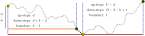
\includegraphics[width=\textwidth]{images/dyck_first_approach_sampling.pdf}
    \caption{Zooming into the error in Figure~\ref{fig:dyck_boundary_invariant}}
    \label{fig:dyck_first_approach_sampling}
\end{figure}

We will parameterize the position $x$ the number of up-steps between $x_i$ and $x$
(See Figure~\ref{fig:dyck_first_approach_sampling}).
This quantity will be referred to as $d$ such that $x - x_{i+1} = 2d + k-1$.
Given a specific $d$, we want to compute the number of valid paths that result in
$d$ up-steps before the first approach to the boundary.
We will calculate this quantity by counting the total number of paths to the left and right
of the first approach and multiplying them together.

Since we only care about getting a asymptotic (up to $\poly(\log n)$ factors) estimate of the probabilities,
it suffices to estimate the number of paths asymptotically as well.

\begin{restatable}{lemma}{ReturnDLeftBound}
\label{lem:ReturnDLeftBound}
If $d > \log^4 n$, then $D_{left}(d)
= \Theta\left( \frac{2^{2d+k}}{\sqrt{d}}\mathlarger e^{-r_{left}(d)}\cdot \frac{k-1}{d+k-1}\right)$
where $r_{left}(d) = \frac{(k-2)^2}{2(2d+k-2)}$.
\end{restatable}
\todo{Deal with smaller values of $d$}

\begin{restatable}{lemma}{ReturnDRightBound}
\label{lem:ReturnDRightBound}
If $U+D-2d-k > \log^4 n$, then $D_{right}(d)
= \Theta\left( \frac{2^{U+D-2d-k}}{\sqrt{U+d-2d-k}}\mathlarger e^{-r_{right}(d)}\cdot \frac{U-D+k}{U-d+1}\right)$
where $r_{right}(d) = \frac{(U-D-k-1)^2}{4(U+D-2d-k+1)}$.
\end{restatable}
\todo{Deal with other values of $d$}


\subsubsection{Estimating the CDF}%
\label{sec:estimating_the_cdf}

\begin{restatable}{lemma}{ReturnProbabilityBoundNotNormalized}
\label{lem:ReturnProbabilityBoundNotNormalized}
$D_{left}(d)\cdot D_{right}(d)
= \Theta\left( \frac{2^{U+D}}{\sqrt{d(U+D-2d-k)}}\mathlarger e^{-r(d)}\cdot\frac{k-1}{d+k-1}\cdot\frac{U-D+k}{U-d+1}\right)$
where $r(d)=\mathcal O(\log^2 n)$.
\end{restatable}
\begin{proof}
This follows from the fact that both $r_{left}(d)$ and $r_{right}(d)$ are $\mathcal O(\log^2 n)$.
\end{proof}

\begin{corollary}
\label{cor:ReturnProbabilityRounding}
The probability $p_d$ of sampling $d$ as the number of up-steps
before the first approach to the boundary can be approximated as:
\[
p_d = \Theta\left( \frac{ 2^{U+D}\cdot\frac{(k-1)(U-D+k)}{\sqrt{d(U+D-2d-k)}(d+k-1)(U-d+1)}\cdot
\mathlarger e^{-\floor{r(d)}} }{\binom{U+D}{U}-\binom{U+D}{D-k}} \right)
\]
\todo{$D_{total}$ is not correct}
This is because the floor function only affects the value of the exponential by a factor of at most $e$.
\end{corollary}
\begin{corollary}
\label{cor:ReturnProbabilityPiecewiseContinuous}
We define a piecewise continuous function
\[
\hat q(d) = \frac{ 2^{U+D}\cdot\frac{(k-1)(U-D+k)}{\sqrt{d(U+D-2d-k)}(d+k-1)(U-d+1)}\cdot
\mathlarger e^{-\floor{r(d)}} }{\binom{U+D}{U}-\binom{U+D}{D-k}}
\]
We claim that $p_d = \Theta\left( \int\limits_d^{d+1} \hat q(d)\right)$.
Note that this integral has a closed form for a fixed value of $\floor{r(d)}$.
\end{corollary}


Let the maximum value of $r(d)$ be $r_{max} = \mathcal O(\log^2 n)$.
\begin{corollary}
\label{cor:}
We can compute the approximate normalized probabilities
\[
q_d = \frac{\int\limits_d^{d+1} \hat q(d)}{\int\limits_1^{n} \hat q(d)}
\]
such that $p_d = \Theta(q_d)$.
Furthermore, we can also compute the CDF of $q_d$ as:
\[
Q_d = \frac{\int\limits_1^{d+1} \hat q(d)}{\int\limits_1^{n} \hat q(d)}
\]
This allows us to sample from the distribution $q_d$ and use Lemma~\ref{lem:huge} to indirectly sample from $p_d$.
\end{corollary}
\todo{Needs a theorem}
\begin{theorem}
\label{thm:first_return_in_interval}
Kinesthetics
\end{theorem}



\subsubsection{Finding the Correct Interval: $\func{First-Return}$ Query}
As before, consider all positions that have been queried already $ \langle x_1, x_2,\cdots, x_m \rangle$ (in increasing order)
along with their corresponding heights $ \langle h_1, h_2,\cdots, h_m \rangle$.
\begin{restatable}{lemma}{FirstReturnInterval}
\label{lem:first_return_interval}
For any position $x_i$, assuming that Proposition~\ref{prop:boundary_invariant} holds,
we can find the interval $(x_{k-1},x_{k}]$ that contains $\func{First-Return}(x_i)$
We do this by by setting $k$ to be either the smallest index $f>i$ such that $h_f\le h_i$ or setting $k=i+1$.
\end{restatable}
\begin{proof}
We assume the contrary i.e. there exists some $k\not=f$ and $k\not=i+1$ such that the correct interval is $(x_{k-1},x_k]$.
Since $h_f<h_i$, the position of first return to $h_i$ happens in the range $(x_i,x_f]$.
So, the only possibility is $i+1 < k \le f-1$.
By the definition of $h_f$, we know that both $h_k$ and $h_{k-1}$ are strictly larger than $h_i$.
Proposition~\ref{prop:boundary_invariant} implies that the boundary for this interval $(h_{k-1},h_k]$ is at $\min(h_{k-1},h_k) > h_i$.
So, it is not possible for the first return to be in this interval.
\end{proof}

The good news is that there are only two intervals that we need to worry about.
Now the challenge is to find the smallest index $f>i$ such that $h_f\le h_i$.
One solution is to maintain an interval tree \todo{cite} over the range $[2n]$ storing the position of the boundary.
Specifically, we have a balanced binary tree with $2n$ leaves with the $i^{th}$ leaf storing the boundary at position $i$.
Each internal node stores the minimum value amongst all the leaves in its sub-tree.
In this setting, we can binary search for $f$ by guessing a bound $f'$ and performing a \emph{range minimum query} over the interval $(x_i,x_{f'}]$.
Overall, this requires $\mathcal O(\log n)$ range queries each of which makes $\mathcal O(\log n)$ probes to the binary tree.

However, we cannot explicitly maintain or even construct this tree, and updates can be as expensive as $\Theta(n)$.
To mitigate this, we start with just a root node (indicating that the initial boundary is $1$ everywhere) and build the tree dynamically as needed.
We perform updates using \emph{lazy propagation} \todo{cite} by only propagating updates down to the children (creating children if necessary) when needed.
So, at any given time, some nodes in the tree may not hold the correct value, but the correct value must be present on the path to the root.
\todo{This probably needs more explanation}

\begin{theorem}
\label{thm:dyck_first_return_sampling}
There is an algorithm using $\mathcal O(poly(\log n))$ resources per query that provides sample access to a Dyck path of length $2n$
by answering queries of the form \func{First-Return}$(x_i)$ with the correctly sampled position $y$;
where $y>x_i$ is the position where the Dyck path first returns to $\func{Height}(x_i)$ after position $x_i$.
\end{theorem}
\begin{proof}
We first query the interval $(x_i,x_{i+1}]$ to find a first return using Theorem~\ref{thm:first_return_in_interval}.
If a return is not found, we calculate $f$ using \todo{what?}.
Since $x_{f-1}<x_i\le x_f$ by definition, the interval $(x_{f-1},x_f]$ must contain a position at height $h_i$.
We sample a point in the middle of this interval and fix the boundary invariant by sampling another point,
essentially breaking it up into $\mathcal O(1)$ sub-intervals each at most half the size of the original.
Based on the new samples, we find the sub-interval containing the first return in $\mathcal O(1)$ time.
We repeat up to $\mathcal O(\log n)$ times until the current interval size drops below the threshold $\mathcal T$.
Then we spend $\tilde{\mathcal O}(\mathcal T)$ time to brute force sample this interval and find the first return position (if it wasn't revealed in previous steps).
\end{proof}
